\section{Introduction}\label{introduction}

\begin{frame}{Caveat Emptor}

I'm not endorsing Bash for large-scale projects, difficult or
performance critical tasks. If your project needs to talk to a database,
object store, interact with a filesystem or dynamically handle block
devices - you \textbf{SHOULD NOT} use Bash in the first place. You can.
But you'll regret it - I speak from years of experience doing completely
insane stuff in Bash for fun (certainly not for profit).

\vfill
Bash is useful for one thing and one thing only: as \emph{glue}!

\vfill

..and it's the glue that holds Linux distributions, Embedded Appliances
and even Commercial networking gear together - so you better use the
best glue on the market, right?

\end{frame}

\begin{frame}{Do we really need another style guide?}

\begin{itemize}
\itemsep1pt\parskip0pt\parsep0pt
\item
  For starters: It's not only a style guide, but more on that later.
\item
  A lot of the internet actually runs on poorly written Bash.
\item
  Your company probably depends on a lot of Bash-glue.
\item
  Everyone uses it on a daily basis to glue userland utilities together.
\item
  Some scripts unintentionally look like they are submissions for an
  obfuscated code contest.
\item
  There are some style guides (e.g.~by Google) and tutorials - but
  nothing definitive.
\item
  Most books on the subject are ancient and often reflect personal
  opinions of authors, outdated Bash versions and userland utilities and
  most haven't been updated in decades.
\item
  I don't know a single good book on Bash. The best resource is still
  \url{http://wiki.bash-hackers.org}.
\end{itemize}

\end{frame}

\section{Working towards a community style
guide}\label{working-towards-a-community-style-guide}

\begin{frame}{Working towards a community style guide}

\begin{itemize}
\itemsep1pt\parskip0pt\parsep0pt
\item
  I've started collecting style guides, tutorials, write-ups, tools and
  debugging projects during the last couple of years.\\ ..chose the best
  ideas and clearest styles and combined them into one big community
  driven effort.
\item
  People started contributing.
\item
  Nothing is written in stone. Come up with a better idea for a certain
  topic and I'll gladly accept it.
\item
  I've also included a lot of mistakes people do or even rely on when
  writing their (often production) scripts.
\item
  I've also collected a lot of tricks and shortcuts I've learned over
  the years specific to bash scripting and the Linux userland.
\end{itemize}

\end{frame}

\section{Doing it wrong}\label{doing-it-wrong}

\begin{frame}{Bad Example}

Here's a cool and bad example at the same time. \texttt{rpm2cpio}
reimplemented in bash.

\begin{itemize}
\itemsep1pt\parskip0pt\parsep0pt
\item
  As Debian package: \texttt{Installed-Size: 1044}
\item
  As Bash script: \texttt{4}
\end{itemize}

\end{frame}

\begin{frame}{Bad Example (cont.)}

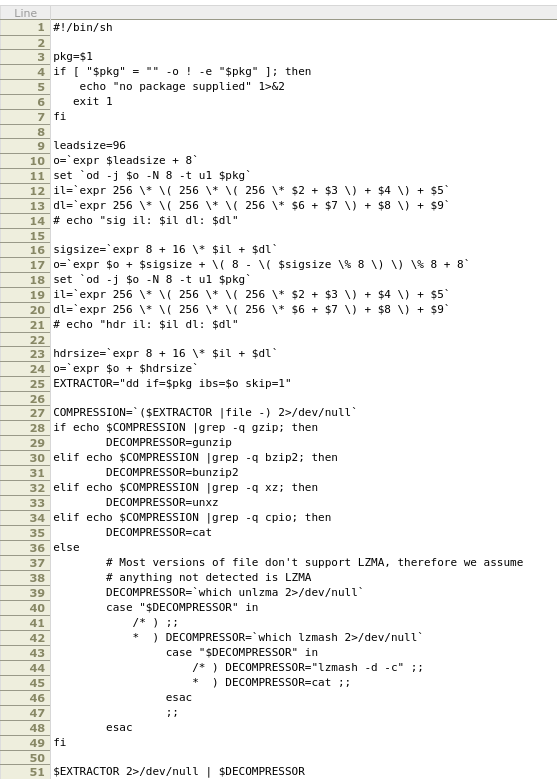
\includegraphics[height=200px]{rpm2cpio}

\tiny
\url{https://trac.macports.org/attachment/ticket/33444/rpm2cpio}

\end{frame}

\begin{frame}{Common bad style practices}

\begin{itemize}
\itemsep1pt\parskip0pt\parsep0pt
\item
  overusing \texttt{grep} for tasks that Bash can do by itself.
\item
  using bourne-shell backticks instead of \texttt{\$()} for subshell
  calls.\\ .. ever tried to nest backtick subshells? yea. you'll have to
  escape them. instead of e.g.:\\
  \texttt{\$(util1 \$(util2 \$\{some\_variable\_as\_argument\}))}.
\item
  manual argument parsing instead of using the \texttt{getopts} builtin.
\item
  using \texttt{awk} for arithmetic operations bash can do very well.\\
  .. same goes for \texttt{expr(1)}. please stop using it in bash
  scripts.\\ .. same goes for \texttt{bc(1)}. please stop using it in
  bash scripts.
\end{itemize}

\end{frame}

\begin{frame}{Common bad style practices (cont.)}

\begin{itemize}
\itemsep1pt\parskip0pt\parsep0pt
\item
  using the \texttt{echo} builtin where \texttt{printf} can (and
  probably should) be used.
\item
  using \texttt{seq 1 15} for range expressions instead of
  \texttt{\{1..15\}}
\item
  many \texttt{coreutils} you do not need \& you save on subshell
  calls.\\ .. a lot is set as a variable in your environment already\\
  (protip: see what \texttt{env} gives you to work with in the first
  place)
\item
  worst of all: endless and unreadable pipe
  glue\ldots{}\ldots{}\ldots{}\ldots{}
\end{itemize}

\end{frame}

\begin{frame}[fragile]{Common bad style practices (cont.)}

So what is more readable to you and probably the angry sysadmin that
might take over your codebase at some point in time? \vspace{20px}

\texttt{ls \$\{long\_list\_of\_parameters\} \textbar{} grep \$\{foo\} \textbar{} grep -v grep \textbar{} pgrep \textbar{} wc -l \textbar{} sort \textbar{} uniq}
\newline
\newline
or

\begin{verbatim}
ls ${long_list_of_parameters}   \
    | grep ${foo}               \
    | grep -v grep              \
    | pgrep                     \
    | wc -l                     \
    | sort                      \
    | uniq
\end{verbatim}

\end{frame}

\begin{frame}{}

\end{frame}

\begin{frame}{Debugging is a mess}

One of the reasons nobody should aim for big projects in Bash is that it
is terrible to debug, most of you will know this already. \vfill

This project aims to make it easier for you to debug your scripts. By
writing beautiful, solid and testable code.

\end{frame}

\section{Modern Bash scripting (Welcome to
2014!)}\label{modern-bash-scripting-welcome-to-2014}

\begin{frame}{Modern Bash scripting}

Most people don't know that there are a lot of useful paradigms and
tools that are used for software engineering in serious languages
available also to Bash.

\vfill
Let's not kid ourselves: some Bash scripts will run in production, even
for years. They'd better work. And not take your business offline.

\end{frame}

\begin{frame}{Test Driven Development and Unit tests with Bash}

\begin{enumerate}
\def\labelenumi{\arabic{enumi}.}
\itemsep1pt\parskip0pt\parsep0pt
\item
  Sam Stephenson (of \texttt{rbenv} fame) wrote an automated testing
  system for Bash scripts called `bats' using TAP (Test Anything
  Protocol): \url{https://github.com/sstephenson/bats}
\item
  \texttt{Sharness}: another TAP library. there's even a Chef cookbook
  for it: \url{https://github.com/mlafeldt/sharness}
\item
  \texttt{Cram}: a functional testing framework based on Marcurial's
  unified test format - \url{https://bitheap.org/cram/}
\item
  \texttt{rnt}: Automated testing of commandline interfaces -
  \url{https://github.com/roman-neuhauser/rnt}
\item
  \texttt{shUnit2}: is a xUnit framework (similar to PyUnit, JUnit et
  cetera) - \url{https://code.google.com/p/shunit2/}
\item
  \texttt{shpec}: Tests/Specs - \url{https://github.com/rylnd/shpec}
\end{enumerate}

..there are more, but these I've found to be most useful.

\end{frame}

\begin{frame}{Linting}

\begin{itemize}
\itemsep1pt\parskip0pt\parsep0pt
\item
  A online Bash style linter:
  \url{https://github.com/koalaman/shellcheck}
\item
  Ubuntu ships with a tool called \texttt{checkbashisms} based on
  Debians \texttt{lintian} (portability).
\item
  \texttt{shlint} tests for portability between zsh, ksh, bash, dash and
  bourne shell (if need be): \url{https://github.com/duggan/shlint}
\item
  For Node fans: Grunt task that checks if a Bash script is valid (not
  anything else, btw):
  \url{https://www.npmjs.com/package/grunt-lint-bash}
\end{itemize}

\end{frame}

\begin{frame}{Inter-shell portability}

\begin{block}{Personal opinion:}

Inter-shell portability doesn't matter. I've spent years writing OS
agnostic bourne-shell scripts. Today every modern OS ships with a
reasonably recent version of Bash. These days Solaris (and FOSS forks
like SmartOS) ship even with a GNU userland. Use Bash.

I love \texttt{zsh} and it can do a lot more. I still use Bash for
(semi-) production scripts. They run basically everywhere when done
right.

\end{block}

\end{frame}

\begin{frame}{Defensive Bash programming}

\begin{itemize}
\itemsep1pt\parskip0pt\parsep0pt
\item
  As you would in every other language, write helper functions, test
  these functions.
\item
  Set constants \texttt{readonly}.
\item
  Write concise, well defined and tested functions for every action.
\item
  Use the \texttt{local} keyword for function-local variables.
\item
  Prepend every function with the \texttt{function} keyword.
\item
  Return proper error codes and check for them.
\item
  Write unit tests.
\item
  Some people write a \texttt{function main()} as people would with
  Python. So one can import and test ones \texttt{main} call as well.
\end{itemize}

\end{frame}

\begin{frame}[fragile]{Defensive Bash programming (cont.)}

\begin{verbatim}
function fail() {
  local msg=${@}

  # handle failure appropriately
  cleanup && logger "my message to syslog"

  echo "ERROR: ${msg}"
  exit 1
}
\end{verbatim}

et cetera

\end{frame}

\begin{frame}[fragile]{Defensive Bash programming (cont.)}

\begin{verbatim}
function linux_distro() {
  local releasefile=$(cat /etc/*release* 2> /dev/null)
  case ${releasefile} in
  *Debian*)             printf "debian\n" ;;
  *Suse*)               printf "sles\n"   ;;
  *CentOS* | *RedHat*)  printf "el\n"     ;;
  *)                    return 1          ;;
  esac
}

...
[[ $(linux_distro) ]] || fail "Unkown distribution!"
readonly linux_distro=$(linux_distro)
...
\end{verbatim}

\end{frame}

\begin{frame}[fragile]{Defensive Bash programming (cont.)}

\begin{verbatim}
function debian_version() {
  # convert debian version to single unsigned integer
  local dv=$(printf "%.f" $(</etc/debian_version))
  printf "%u" ${dv}
}
\end{verbatim}

\end{frame}

\begin{frame}[fragile]{Defensive Bash programming (cont.)}

\begin{verbatim}
function is_empty() {
  local var=${1}
  [[ -z ${var} ]]
}

function is_file() {
  local file=${1}
  [[ -f ${file} ]]
}

function is_dir() {
  local dir=${1}
  [[ -d ${dir} ]]
}
\end{verbatim}

\end{frame}

\begin{frame}[fragile]{Signal Handling}

\begin{itemize}
\itemsep1pt\parskip0pt\parsep0pt
\item
  Bash supports signal handling with the builtin \texttt{trap}:
\end{itemize}

\begin{verbatim}
# call the fail() function if one
# of these signals is caught by trap:
trap 'fail "caught signal!"' HUP KILL QUIT
\end{verbatim}

\end{frame}

\begin{frame}[fragile]{Anonymous Functions (Lambdas)}

You'll probably never ever need this in Bash, but it's possible:

\begin{verbatim}
function lambda() {
  _f=${1} ; shift
  function _l {
    eval ${_f};
  }
  _l ${*} ; unset _l
}
\end{verbatim}

\end{frame}

\begin{frame}{Bash Profiling}

\begin{itemize}
\itemsep1pt\parskip0pt\parsep0pt
\item
  Sam Stephenson also wrote a profiler for Bash scripts:
  \url{https://github.com/sstephenson/bashprof}
\end{itemize}

\end{frame}

\begin{frame}{Bash Debugging}

Hopefully you'll write code that you do not have to debug often, but
eventually you'll have to. There's only one real way to debug a Bash
script unfortunately:

\begin{itemize}
\itemsep1pt\parskip0pt\parsep0pt
\item
  \texttt{bash -evx script.sh}
\item
  or setting \texttt{set -evx} in your script directly
\item
  that being said, someone wrote a Bash debugger with \texttt{gdb}
  command syntax: \url{http://bashdb.sourceforge.net/}
\end{itemize}

\end{frame}

\section{Conclusion}\label{conclusion}

\begin{frame}{Conclusion}

\begin{itemize}
\itemsep1pt\parskip0pt\parsep0pt
\item
  There's a lot more to tell (just ask me afterwards) - but this was
  supposed to be a lightning talk.
\item
  All this, a lot of references and other projects are mentioned in my
  \texttt{Community Bash Style Guide} which is on GitHub.
\item
  Please contribute in any way you can if you come up with useful
  Bashisms, tricks or find any cool projects.
\item
  Any input is very much appreciated!
\end{itemize}

\begin{block}{Fork and open Pull Requests, Issues or Complaints!}

\url{https://github.com/azet/community_bash_style_guide}

\end{block}

\end{frame}
